\newpage
\begin{center}
  \textbf{
  \MakeUppercase{Приложение А}\\
  (обязательное)\\
  \vspace{1em}
  Исходный код}
  \end{center}
  \addcontentsline{toc}{section}{Приложение А (обязательное) Исходный код}
  
  \lstinputlisting[style=js]{appendices/index.js}
  \lstinputlisting[style=js]{appendices/App.js}
  \begin{center}
    Продолжение приложения А
    \end{center}
  \lstinputlisting[style=js]{appendices/src/dialog.js}
  
  \newpage

  \begin{center}
    \textbf{
      \MakeUppercase{Приложение Б}\\
      (обязательное)\\
      \vspace{1em}
      Отчет о проверке на заимствования}
    \end{center}
    \addcontentsline{toc}{section}{Приложение Б (обязательное) Отчет о проверке на заимствования}
    \begin{figure}[h]
      \centering
      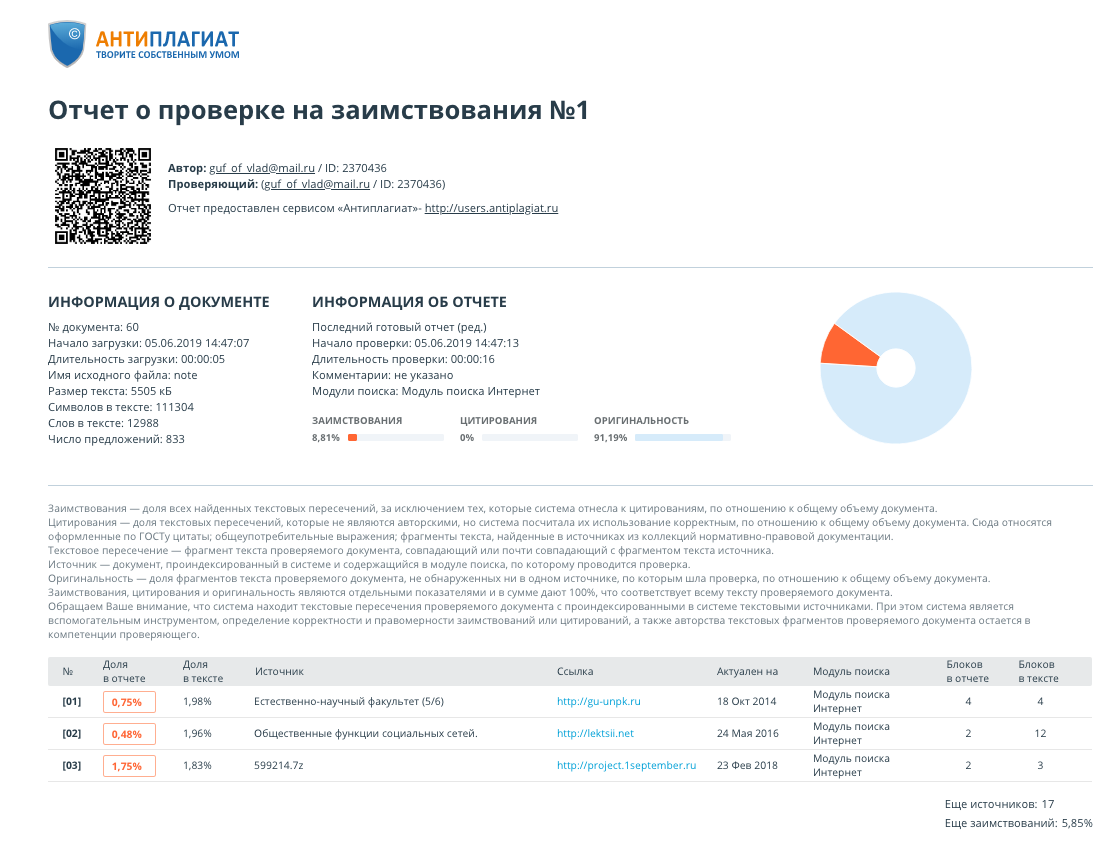
\includegraphics[scale=0.42]{antiplagiat.png} 
    \end{figure}
    \vspace{-5mm}
      \centerline{Рисунок Б -- Отчет о проверке на заимствования}
    
    \newpage
  
  \begin{center}
  \textbf{
  \MakeUppercase{Приложение В}\\ 
  (справочное)\\
  \vspace{1em}
  Описание схемы базы данных}
  \end{center}
  \addcontentsline{toc}{section}{Приложение В (справочное) Описание схемы базы данных}
  
  \lstinputlisting[style=fsharpstyle]{appendices/db_schema1.ndef}
  \begin{center}
    Продолжение приложения В
    \end{center}
  \lstinputlisting[style=fsharpstyle]{appendices/db_schema2.ndef}
  \begin{center}
    Продолжение приложения В
    \end{center}
  \lstinputlisting[style=fsharpstyle]{appendices/db_schema3.ndef}

  \newpage
  
  \begin{center}
  \textbf{
  \MakeUppercase{Приложение Г}\\
  (справочное)\\
  \vspace{1em}
  Конфигурационные файлы проекта}
  \end{center}
  \addcontentsline{toc}{section}{Приложение Г (справочное) Конфигурационные файлы проекта}
  
  \lstinputlisting[style=js]{appendices/.eslintrc}
  \newpage
  \begin{center}
    Продолжение приложения Г
    \end{center}
  \lstinputlisting[style=js]{appendices/package.json}